\section{Experimental Setup}

The submitted solution consists of three final pipelines: \texttt{Schema-RAG}, \texttt{Reasoned-RAG}, and \texttt{Mixed-SC}. These correspond to the submitted names \path{enriched-schema-rag}, \path{enriched-inline-reasoning-rag}, and \path{mixed-extractors-self-consistency-rag}. We also report a non-RAG baseline for comparison.

The results below are computed from our final test-set run logs rather than from an official leaderboard release. They cover 145 test instances evaluated with two hosted models exposed through an OpenAI-style chat interface: \path{google_gemma-4-e4b-it} and \path{qwen/qwen3-14b}. Baseline, \texttt{Schema-RAG}, and \texttt{Mixed-SC} were run with both models; the available \texttt{Reasoned-RAG} run uses Gemma only. The GenSIE overview paper remains the authoritative source for dataset construction, official ranking, model selection, and shared-task scoring details \cite{gensie2026overview}.

We report micro-averaged precision, recall, and \(F_1\) by summing the evaluator's true-positive mass, gold keys, and system keys over a subset before computing the metric. Token counts are the average total input-plus-output tokens per instance from the run logs. We do not report wall-clock-time comparisons: the logs do not provide enough granular traceability to separate our code from hosted backend latency and small-language-model generation delays inside the evaluation service. We also report \texttt{calls=0}, the number of instances for which no model call was completed; these cases contribute no true positives and explain much of the gap between all-instance and nonzero-call analyses.

The test set contains 23 unique schema fingerprints under the same structural normalization used by retrieval. Ten fingerprints are present in the development/FSP corpus, but they account for only 36 of 145 test instances. The remaining 13 unseen fingerprints account for 109 instances. Before the test set was released, the task description suggested a roughly balanced mixture of seen and unseen schemas; this influenced the design toward supporting both exact same-schema reuse and complementary field-level fallback. The final test distribution is more skewed toward unseen-schema instances, making the fallback route more central than expected.

\section{Results and Analysis}

Table~\ref{tab:main-results} shows the aggregate runs. Since the two models have different baselines, raw \(F_1\) is not by itself a representative cross-model comparison. We therefore also report the fraction of the baseline-to-1.0 \(F_1\) gap closed by each non-baseline run, \((F_1^{system}-F_1^{baseline})/(1-F_1^{baseline})\), computed within the same model. Accordingly, the analysis emphasizes gap closed relative to each model's baseline rather than absolute \(F_1\) alone. For both models, \texttt{Schema-RAG} closes a substantial part of the baseline gap. With Gemma, \texttt{Schema-RAG} obtains the highest aggregate \(F_1\) among the available Gemma runs, while \texttt{Reasoned-RAG} is close but slightly lower. With Qwen, \texttt{Mixed-SC} gives the best aggregate \(F_1\), narrowly ahead of \texttt{Schema-RAG}, but at much higher token cost.

\begin{table}[!htbp]
\centering
\caption{Test-set metrics from final run logs. Tokens are average total tokens per instance. Gap is the fraction of the model-specific baseline-to-1.0 \(F_1\) gap closed.}
\label{tab:main-results}
\scriptsize
\begin{tabular}{@{}llrrrrrr@{}}
\toprule
Model & Pipeline & Prec. & Rec. & \(F_1\) & Gap & Tok. & \texttt{calls=0} \\
\midrule
Gemma & Baseline & 0.702 & 0.639 & 0.669 & -- & 3691 & 18 \\
Gemma & \texttt{Schema-RAG} & 0.805 & 0.699 & 0.748 & 23.9\% & 4904 & 18 \\
Gemma & \texttt{Reasoned-RAG} & 0.807 & 0.691 & 0.744 & 22.8\% & 8137 & 18 \\
Gemma & \texttt{Mixed-SC} & 0.807 & 0.689 & 0.743 & 22.4\% & 13670 & 20 \\
\midrule
Qwen & Baseline & 0.699 & 0.590 & 0.640 & -- & 3671 & 18 \\
Qwen & \texttt{Schema-RAG} & 0.793 & 0.683 & 0.734 & 26.1\% & 5047 & 20 \\
Qwen & \texttt{Mixed-SC} & 0.800 & 0.702 & 0.747 & 29.8\% & 12688 & 18 \\
\bottomrule
\end{tabular}
\end{table}

Figure~\ref{fig:main-result-bars} visualizes the same aggregate results. The left panel emphasizes the baseline-normalized view: \texttt{Schema-RAG} closes a similar fraction of the available gap for both models, while Qwen \texttt{Mixed-SC} closes the largest fraction but with the token cost shown in Table~\ref{tab:main-results}. The right panel keeps the raw precision, recall, and \(F_1\) values visible for each model-pipeline pair.

\begin{figure}[!htbp]
\centering
\begin{minipage}[t]{0.44\linewidth}
\centering
\begin{tikzpicture}
\begin{axis}[
  ybar,
  width=\linewidth,
  height=0.22\textheight,
  ymin=0,
  ymax=34,
  ylabel={Gap closed (\%)},
  symbolic x coords={S-RAG,R-RAG,Mixed-SC},
  xtick=data,
  xticklabel style={font=\scriptsize},
  yticklabel style={font=\scriptsize},
  label style={font=\scriptsize},
  legend style={
    font=\scriptsize,
    at={(0.5,1.03)},
    anchor=south,
    legend columns=2,
    draw=none
  },
  bar width=8pt,
  enlarge x limits=0.28,
  nodes near coords,
  nodes near coords style={font=\tiny},
  every node near coord/.append style={
    /pgf/number format/fixed,
    /pgf/number format/precision=1
  }
]
\addplot coordinates {(S-RAG,23.9) (R-RAG,22.8) (Mixed-SC,22.4)};
\addplot coordinates {(S-RAG,26.1) (Mixed-SC,29.8)};
\legend{Gemma,Qwen}
\end{axis}
\end{tikzpicture}
\end{minipage}\hfill
\begin{minipage}[t]{0.53\linewidth}
\centering
\begin{tikzpicture}
\begin{axis}[
  xbar,
  width=\linewidth,
  height=0.22\textheight,
  xmin=0.55,
  xmax=0.84,
  xlabel={Score},
  symbolic y coords={Q-MSC,Q-SR,Q-B,G-MSC,G-RR,G-SR,G-B},
  ytick=data,
  yticklabel style={font=\tiny},
  xticklabel style={font=\tiny},
  label style={font=\scriptsize},
  legend style={
    font=\tiny,
    at={(0.5,1.03)},
    anchor=south,
    legend columns=3,
    draw=none
  },
  bar width=2.2pt,
  enlarge y limits=0.12
]
\addplot coordinates {
  (0.702,G-B) (0.805,G-SR) (0.807,G-RR) (0.807,G-MSC)
  (0.699,Q-B) (0.793,Q-SR) (0.800,Q-MSC)
};
\addplot coordinates {
  (0.639,G-B) (0.699,G-SR) (0.691,G-RR) (0.689,G-MSC)
  (0.590,Q-B) (0.683,Q-SR) (0.702,Q-MSC)
};
\addplot coordinates {
  (0.669,G-B) (0.748,G-SR) (0.744,G-RR) (0.743,G-MSC)
  (0.640,Q-B) (0.734,Q-SR) (0.747,Q-MSC)
};
\legend{Prec.,Rec.,\(F_1\)}
\end{axis}
\end{tikzpicture}
\end{minipage}
\caption{Aggregate result views. Left: fraction of model-specific baseline \(F_1\) gap closed by each non-baseline run. Right: precision, recall, and \(F_1\) by model-pipeline pair. Abbreviations: G/Q = Gemma/Qwen, B = baseline, SR = \texttt{Schema-RAG}, RR = \texttt{Reasoned-RAG}, MSC = \texttt{Mixed-SC}. Qwen \texttt{Reasoned-RAG} was not available.}
\label{fig:main-result-bars}
\end{figure}

\subsection{Retrieval Contribution}

The comparison with the baseline is the clearest available evidence for the usefulness of retrieval, although it is not a controlled ablation of every prompt change. As Table~\ref{tab:component-deltas} shows, \texttt{Schema-RAG} improves \(F_1\) by 0.079 with Gemma and 0.094 with Qwen on all instances, closing 23.9\% and 26.1\% of the respective baseline gaps. When instances with zero calls on either side are removed, the gains increase to 0.094 and 0.119, closing 33.7\% and 38.2\% of the nonzero-call baseline gaps.

\begin{table}[!htbp]
\centering
\caption{Selected component comparisons. ``No zero calls'' excludes instances where either compared run has \texttt{calls=0}. Token deltas are average total tokens per instance. Gap columns are shown only for comparisons against the model-specific baseline.}
\label{tab:component-deltas}
\scriptsize
\begin{tabularx}{\linewidth}{@{}>{\raggedright\arraybackslash}Xrrrrr@{}}
\toprule
Comparison & \(\Delta F_1\) & Gap & No-zero \(\Delta F_1\) & No-zero gap & \(\Delta\) tok. \\
\midrule
Gemma: \texttt{Schema-RAG} vs. baseline & +0.079 & 23.9\% & +0.094 & 33.7\% & +1213 \\
Qwen: \texttt{Schema-RAG} vs. baseline & +0.094 & 26.1\% & +0.119 & 38.2\% & +1376 \\
Gemma: \texttt{Mixed-SC} vs. \texttt{Schema-RAG} & -0.005 & -- & +0.004 & -- & +8766 \\
Qwen: \texttt{Mixed-SC} vs. \texttt{Schema-RAG} & +0.013 & -- & +0.006 & -- & +7641 \\
\bottomrule
\end{tabularx}
\end{table}

The retrieval-only replay selected the same-schema route for 36 instances and attempted the field-aware fallback for the remaining 109. Ten fallback instances enter a retrieval-failure path, so the route-level field-RAG comparison below uses the 99 instances with complete field-embedding diagnostics. This split aligns with the seen/unseen schema split under the structural fingerprint.

\begin{table}[!htbp]
\centering
\caption{Performance by retrieval route. Same-schema contains 36 instances; Field-RAG contains the 99 fallback instances with complete field-embedding diagnostics.}
\label{tab:route-performance}
\scriptsize
\begin{tabular}{@{}llrrrrrr@{}}
\toprule
& & \multicolumn{3}{c}{Same-schema} & \multicolumn{3}{c}{Field-RAG} \\
\cmidrule(lr){3-5}\cmidrule(l){6-8}
Model & Pipeline & Prec. & Rec. & \(F_1\) & Prec. & Rec. & \(F_1\) \\
\midrule
Gemma & Baseline & 0.639 & 0.667 & 0.653 & 0.725 & 0.693 & 0.709 \\
Gemma & \texttt{Schema-RAG} & 0.765 & 0.737 & 0.751 & 0.830 & 0.756 & 0.791 \\
Gemma & \texttt{Reasoned-RAG} & 0.804 & 0.775 & 0.789 & 0.820 & 0.731 & 0.773 \\
Gemma & \texttt{Mixed-SC} & 0.801 & 0.742 & 0.770 & 0.821 & 0.739 & 0.778 \\
\midrule
Qwen & Baseline & 0.622 & 0.558 & 0.588 & 0.725 & 0.660 & 0.691 \\
Qwen & \texttt{Schema-RAG} & 0.734 & 0.707 & 0.720 & 0.825 & 0.743 & 0.782 \\
Qwen & \texttt{Mixed-SC} & 0.779 & 0.779 & 0.779 & 0.818 & 0.745 & 0.780 \\
\bottomrule
\end{tabular}
\end{table}

\texttt{Schema-RAG} improves over baseline in both routes: with Gemma, \(F_1\) increases by 0.098 on same-schema instances and 0.082 on field-RAG instances; with Qwen, the corresponding gains are 0.132 and 0.091. Figure~\ref{fig:rag-route-delta} shows that same-schema reuse is helpful, but not the only source of gains. Excluding zero-call instances, the field-RAG gains are 0.092 for Gemma and 0.107 for Qwen. These results suggest that retrieval is not only exploiting exact schema reuse; complementary field-level examples also contribute on unseen schemas when the field-aware route completes. Additional retrieval diagnostics are summarized in Appendix~\ref{sec:appendix-retrieval-diagnostics}.

\begin{figure}[!htbp]
\centering
\begin{tikzpicture}
\begin{axis}[
  ybar,
  width=0.58\linewidth,
  height=0.22\textheight,
  ymin=0,
  ymax=0.15,
  ylabel={\(\Delta F_1\) vs. baseline},
  symbolic x coords={Same-schema,Field-RAG},
  xtick=data,
  xticklabel style={font=\scriptsize},
  yticklabel style={font=\scriptsize},
  label style={font=\scriptsize},
  legend style={
    font=\scriptsize,
    at={(0.5,1.03)},
    anchor=south,
    legend columns=2,
    draw=none
  },
  bar width=10pt,
  enlarge x limits=0.35,
  nodes near coords,
  nodes near coords style={font=\tiny},
  every node near coord/.append style={
    /pgf/number format/fixed,
    /pgf/number format/precision=3
  }
]
\addplot coordinates {(Same-schema,0.098) (Field-RAG,0.082)};
\addplot coordinates {(Same-schema,0.132) (Field-RAG,0.091)};
\legend{Gemma,Qwen}
\end{axis}
\end{tikzpicture}
\caption{\texttt{Schema-RAG} \(F_1\) gain over the baseline by retrieval route. Field-RAG includes the 99 fallback instances with complete field-embedding diagnostics.}
\label{fig:rag-route-delta}
\end{figure}

\subsection{Reasoning and Self-Consistency}

\texttt{Reasoned-RAG} was available only for Gemma. Its aggregate \(F_1\) is slightly below \texttt{Schema-RAG} (0.744 vs. 0.748), closes 22.8\% of the baseline gap compared with 23.9\% for \texttt{Schema-RAG}, and uses substantially more tokens. The route-level pattern is mixed: relative to \texttt{Schema-RAG}, reasoning improves the same-schema subset by 0.039 \(F_1\) but is lower by 0.018 on field-RAG instances. A plausible interpretation is that explicit top-level evidence wrappers help when retrieved examples share the exact output contract, but add overhead when the examples are only field-complementary. This should be treated as a diagnostic observation rather than a causal result, because Qwen reasoning runs and controlled reasoning ablations are not yet available.

\texttt{Mixed-SC} does not consistently outperform the strongest single-call extractor. For Gemma it is slightly below \texttt{Schema-RAG} on all instances and only marginally above it after zero-call instances are excluded. For Qwen it improves the aggregate \(F_1\) by 0.013, increasing the gap closed from 26.1\% to 29.8\%, but the nonzero-call gain is only 0.006. The cost is much larger: \texttt{Mixed-SC} adds roughly 7.6K--8.8K average tokens per instance over \texttt{Schema-RAG}. Its main benefit appears in same-schema subsets, where it improves over \texttt{Schema-RAG} by 0.020 with Gemma and 0.059 with Qwen, while it is flat or lower on field-RAG subsets. This supports using self-consistency as a robustness mechanism, but not as a uniformly efficient default.

\subsection{Failure Patterns}

The largest non-semantic failure mode is zero completed model calls. Eighteen such instances are common across the main runs: 10 \texttt{TaxonomicClassification} instances and 8 \texttt{ClinicalTrialRecord} instances. The former coincide with the retrieval-failure path in our replay, while the latter pass retrieval and fail later in execution. A few extra zero-call cases are run-specific, including two in Gemma \texttt{Mixed-SC} and two in Qwen \texttt{Schema-RAG}. Because these failures dominate some schema and route subsets, we report both all-instance metrics and nonzero-call comparisons.

Among successful calls, the systems usually produce fewer keys than the gold output on average. \texttt{Schema-RAG} reduces this gap relative to the baseline in several subsets, but underproduction remains visible in the aggregate. This is consistent with the task's strict grounding requirement: omitting uncertain fields tends to raise precision relative to recall, while array and object fields can lose multiple gold keys when a list item or nested object is missed. A field-level error analysis requires aligned prediction details and is left for future controlled analysis.

We keep several exploratory diagnostics out of the main paper body to avoid overinterpreting non-controlled correlations: per-domain and per-schema tables, selected-example hub analyses, pair-score and coverage tertiles, task-level improvement/regression lists, and wall-clock-time comparisons. The appendix retains only the retrieval diagnostics needed to support the main same-schema versus field-RAG interpretation.
